\documentclass[12pt]{article}
\usepackage[utf8]{inputenc}
\usepackage[citestyle=chicago-authordate,style=authoryear, natbib=true, doi=false,isbn=false,url=false, backend=bibtex]{biblatex}
\renewcommand\nameyeardelim{, }
\usepackage{tikz}
\usepackage{amssymb}
\usepackage{mathrsfs}
\usepackage{booktabs}
\usepackage{dcolumn}
\usepackage{multirow}
\usepackage[english]{babel} % To obtain English text with the blindtext package
\usepackage{blindtext}
\usepackage{csquotes}
\usepackage{amssymb}
\usepackage{CJKutf8}
\usepackage{graphicx}
\usepackage{lscape}
\graphicspath{ {./images/} }
\usepackage[T1]{fontenc}
\usepackage[margin = 1in]{geometry}
\usepackage{url} 
\linespread{1.0}

\title{Cloudy Maps, Clear Classifiers: Comparing Methods of Identifying Clouds Over the Arctic}
\author{Andrew Kenealy (amk117@duke.edu) & Viola Rothschild (vlr14@duke.edu)}
\date{Due: December 6, 2022}

\begin{document}
\maketitle
\section{Data Collection and Exploration}
\subsection{Summary}

The urgency of climate change cannot be overstated. Greenhouse gas concentrations are at their highest levels in 2 million years, and emissions continue to rise. As a result, the Earth is now about 1.1 degrees C warmer than it was in the late 1800s and the last decade (2011-2020) was the warmest on record. The consequences of climate change and global warming are already having catastrophic consequences, such as intense droughts, water scarcity, severe fires, rising sea levels, flooding, melting polar ice, catastrophic storms and declining biodiversity---and the effects are only becoming more severe (United Nations, 2022). The systematic and accurate measurement of climate phenomena is a difficult yet critical step towards attempting to avoid further environmental degradation.  
\newline
\newline 
In this study, Shi et al (2008) tackle an important piece of this challenge by developing sophisticated classification algorithms to detect and categorize cloud coverage in the Arctic---where the strongest dependences of surface air temperatures on increasing atmospheric carbon dioxide levels are taking place. Given the critical location of the polar regions, assessing the properties of Arctic clouds is key to determining whether they are changing in ways that protect against or further exacerbate warming in the Arctic. However, accurately studying the properties of Arctic clouds presents significant challenges, as it is very difficult to distinguish between the liquid and ice particles of clouds with the ice and snow covered surface particles due to similarities in the emissions of infrared electromagnetic radiation (IER). Fortunately, with the launch of the Multiangle Imaging SpectroRadiometer (MISR) aboard a NASA satellite, new data has become available that continuously captures IER measurements at multiple view angles. Shi et al use these data to develop novel methods that improve the accuracy of existing techniques that identify cloud particles.  
\newline
\newline 
The data used by Shi et al were collected over the course of 10 MISR orbits of a single path over the Arctic, spanning approximately 144 days from April 28 through September 19, 2002 (total daylight in the Arctic). The images recorded by MISR are 1.1km-pixels. To evaluate the performance of the algorithms, the pixels were then hand coded by experts and labeled as clear or cloudy, resulting in just over 5 million pixels. Shi et al's central innovation was to identify cloud-free surface pixels in the images, rather than cloudy pixels as in the existing MISR algorithms. Modeling the surface has an advantage over modeling clouds because the surface remains constant across different views, whereas clouds always vary from one view to the next. The authors then demonstrate that three physical features---the linear correlation of radiation measurements from different MISR view directions (CORR), the standard deviation of MISR nadir red radiation measurements within a small region (SDAn), and a normalized difference angular index (NDAI)---contain the requisite information to accurately distinguish between clouds and surface. Finally, using these features, the authors develop two algorithms that use enhanced linear correlation matching (ELCM) and quadratic discriminant analysis (ELCM-QDA) to identify and categorize pixels. Based on testing that leverages over 5 million expert-labeled pixels, both algorithms produce significantly more accurate results than existing classification processes.

\subsection{Exploratory Data Analysis}
Before embarking on our main analysis, we first attempt to understand the basic features of the image data. We show that proportion of expertly labeled pixels that are identified as cloud, no cloud, and unlabeled in Table 1.  

\begin{table}[h!]
\centering
\caption{Expert Labels in Each Image (percent)}
\label{table:1}
 \begin{tabular}{||c c c c||} 
 \hline
 & Cloud & Not Cloud & Unlabeled\\ 
 \hline\hline
 Image 1 & 34.11 & 37.25 & 28.64 \\ 
 Image 2 & 17.77 & 43.78 & 38.46 \\
 Image 3 & 18.44 & 29.29 & 52.27 \\
 \hline
 Total & 23.43 & 36.78 & 39.79 \\ 
 \hline
 \end{tabular}
\end{table}
\noindent Across the three images, 23.43 percent of the pixels are identified as cloud, 36.78 percent as not cloud, and 39.79 percent are left unlabeled. We show the actual images in Figure 1. Clouds are represented as light blue, not clouds as white, and unlabeled as grey. The unlabeled pixels (grey) tend to be buffer regions between cloud and not clouds, indicating that it was difficult to identify precise boundaries. Furthermore, we can see clearly from the images that the data is \textit{not} i.i.d.  
\newline
\begin{figure}[htp]
\caption{Images with Expert Labels}
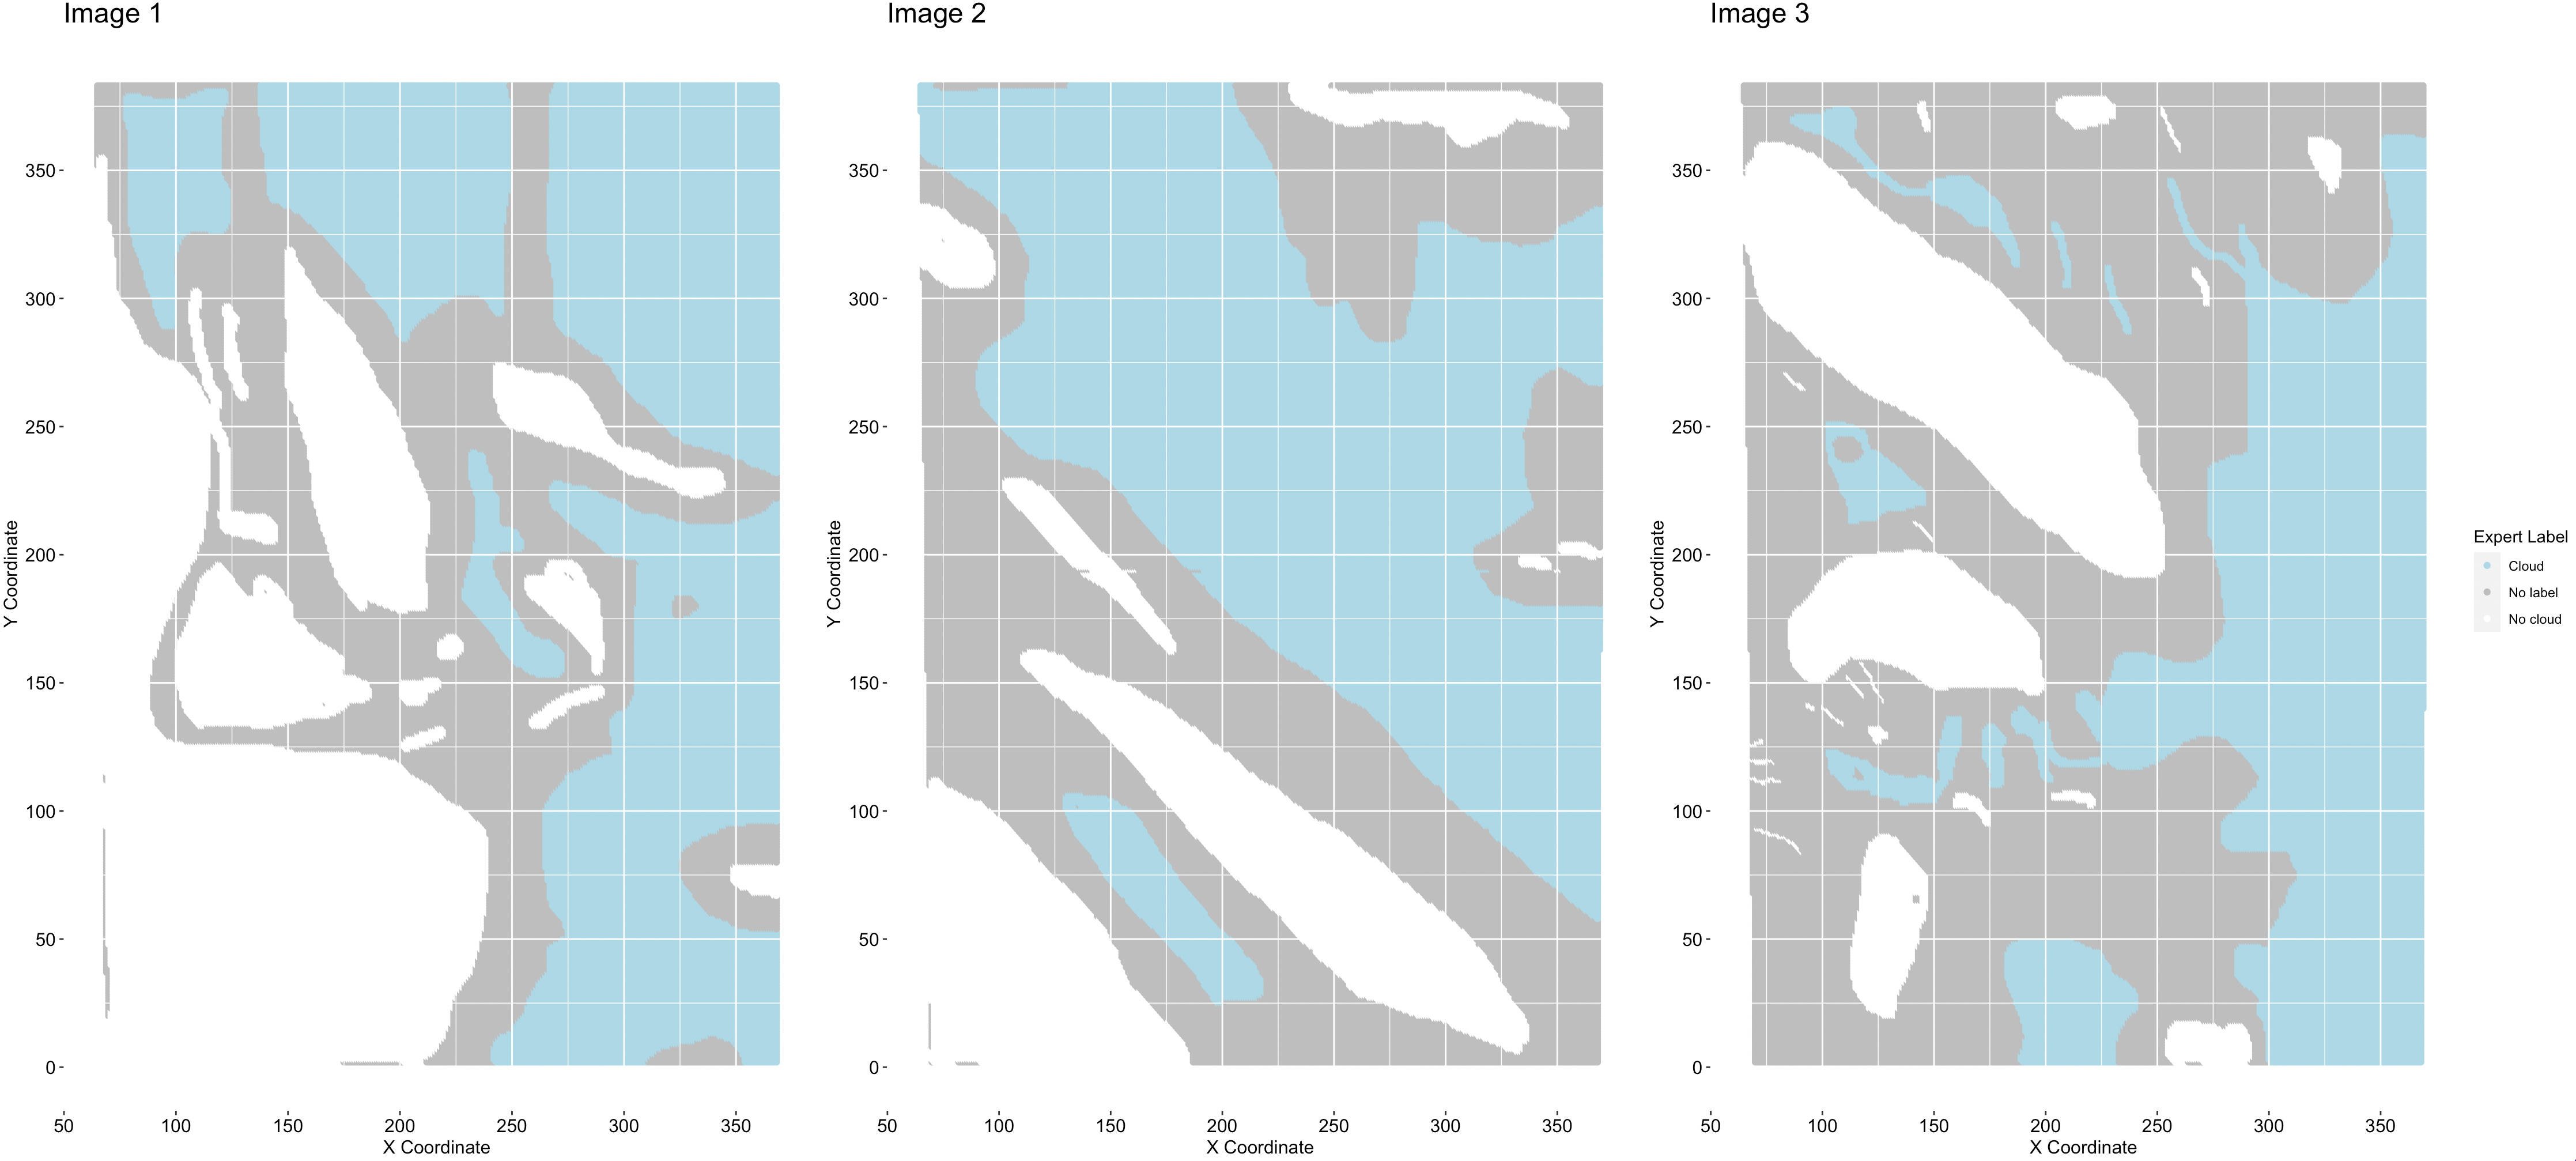
\includegraphics[width=15cm]{Fig1.png}
\centering
\end{figure}

\noindent Next, we conduct a pairwise comparison of the eight different features in the dataset (Figure 2). For this analysis, we remove all unlabeled data points in order to more clearly visualize the relationships between the features and cloud vs. not cloud. We examine three key features computed based on subject knowledge---NDAI (normalized difference angular index), CORR (linear correlation of radiation measurement from the different cameras), and SD (standard deviation of radiation measurement in a small region). Furthermore, the MISR sensor has nine cameras that capture radiance angle information---we analyze data from five of those cameras (DF, CF, BF, AF, and AN). DF, CF, BF, and AF are forward facing cameras in order of decreasing angle direction (and proximity), and AN is the nadir camera pointed directly downwards. For the pairwise comparison, we combine the data from all three images for better representativeness and ease of interpretation. 
\newline
\newline
The relationship between the three subject-knowledge features is difficult to interpret. We see that all pairs of these features are positively correlated with each other, but not strikingly so. NDAI, CORR, and SD are all negatively related to the camera radiance angles, with the exception of CORR and DF (the forward-facing camera at the most extreme angle) which is weakly positive. Generally, as the camera angle becomes more extreme (moving from DF to AF), the correlations become increasingly negative. Examining the relationship between camera radiance angles is more intuitive. We would expect that cameras that are closer together would have a higher correlation. Sure enough, we see that as cameras get further apart, correlation decreases. As expected, the lowest correlation between cameras is with AN, the only nadir facing camera. In terms of the relationship between the features and the expert labels, we see that the no cloud labels (red) tend to be clustered at the extremes (particularly with NDAI), while the could labels (blue) are generally more dispersed (particularly with the radiance angles). 

\begin{figure}[htp]
\caption{Correlation Plot of Features}
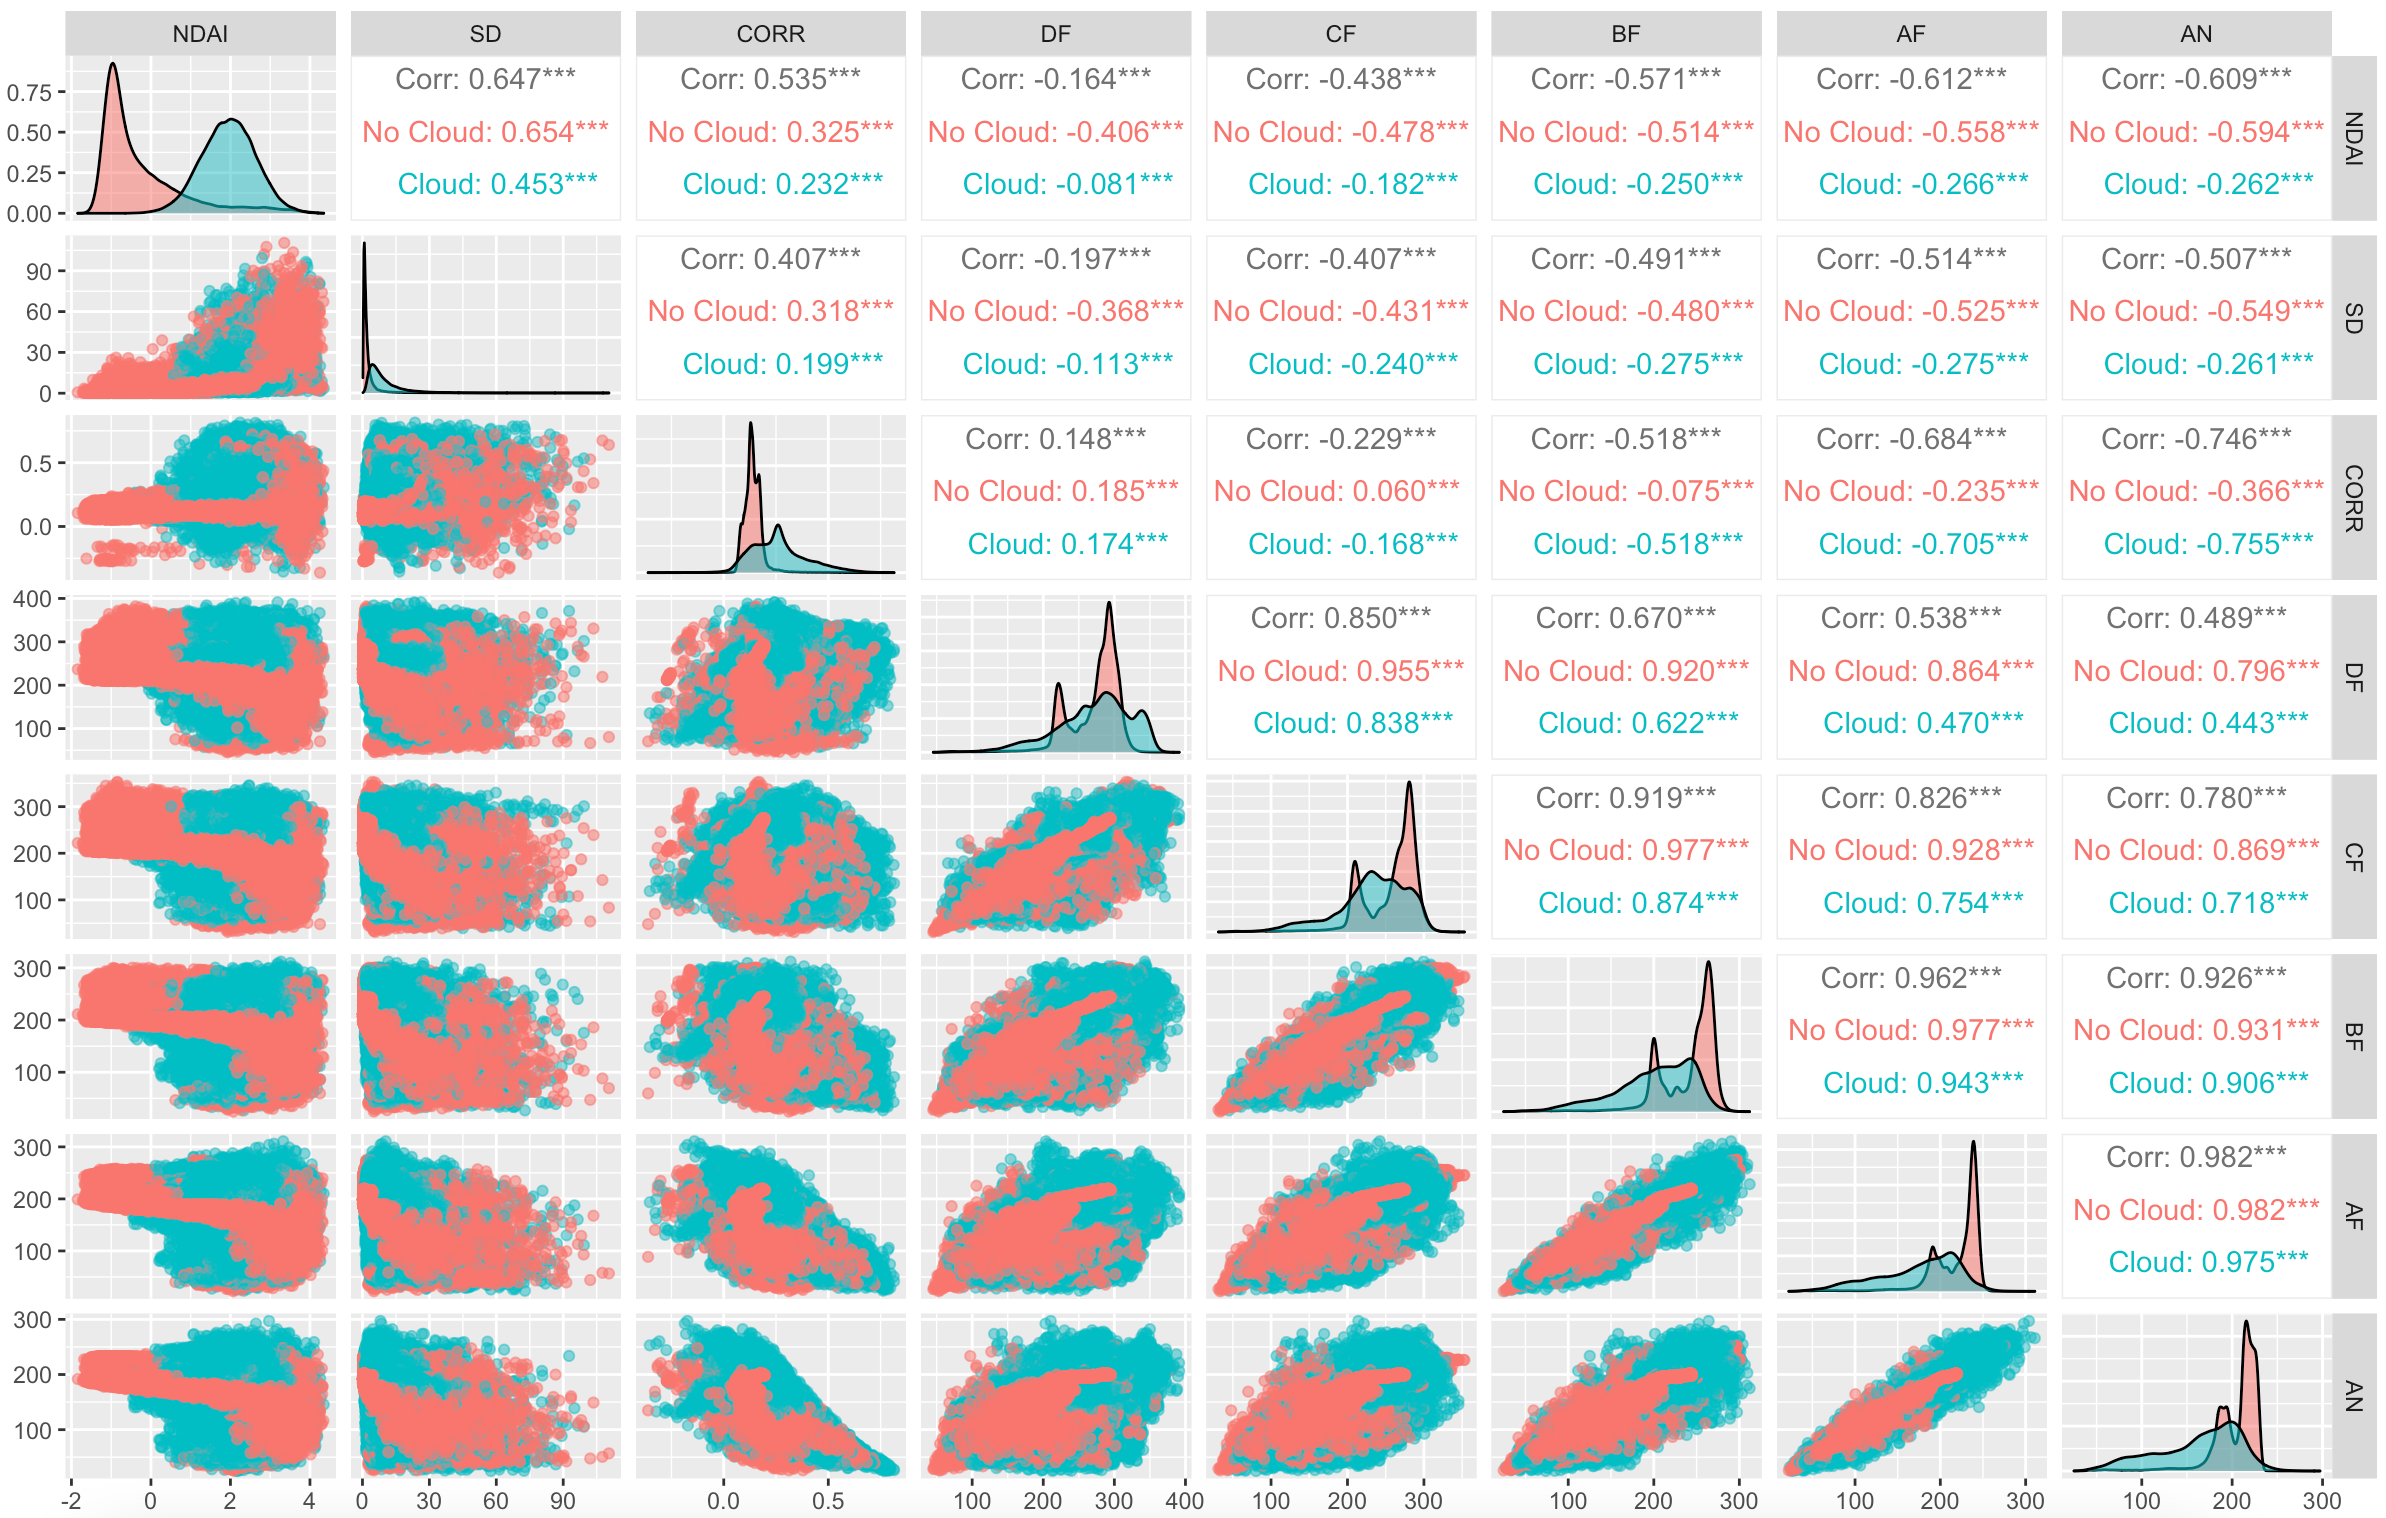
\includegraphics[width=16cm]{Fig2.png}
\centering
\end{figure}

\section{Data Preparation}
\subsection{Data Split}
In order to train and test classification models we must, of course, partition the data into three sets: a training set, a validation set, and a test set. But because this is spatial data, and could and non-cloud datapoints are highly spatially correlated, they are not distributed i.i.d. Thus, predicting the label of a single random datapoint is pretty easy using the labels of other surrounding datapoints (it is likely to be the same as the datapoints around it). This, in turn, means that a trivial random selection of datapoints risks overestimating the true predictive accuracy of a model that is faced with new images. 
\newline
\newline
We utilize two non-trivial partition methods that take into account the spatial correlation of the data.  The first is a horizontal image-slicing partition, the second is a block partition.  We explain each in turn. 
\newline
\newline
Horizontal image slicing divides the dataset into 8 sequential horizontal slices based on the x-y coordinates of each datapoint. One slice is used as the test set, a second as the validation set, and the remaining 6 slices are left for the training data. We select this breakdown (1/8, 1/8, 3/4) based on commonly used ratios of data splitting. 
\newline
\newline
The block partition method divides the data into 64 roughly equally sized squares of data, again based on x-y coordinates. Eight of these blocks (1/8 of the data) are randomly selected to be the test data, another eight blocks are selected to be validation, and the remaining 48 blocks are left as training data. This method has the advantage of randomly capturing regions of data from the images that are from a broader range of both of y and x coordinates, while still preserving some of the spatial structure of the datapoints. Specifically, data in these training, validation, and test sets should have support across the full range of y and x coordinates. This is not true for the horizontal slicing method, which constrains the y-coordinate range of the test and validation data. 

\subsection{Baseline with a Trivial Classifier}
In order to gauge the efficacy of more sophisticated classification methods, we first test a trivial classifier that simply classifies each datapoint as a non-cloud (-1)---the most common label in the dataset.  This trivial classifier correctly classifies about 58 percent of validation and test observations when using the block partition and about 49 percent when using the horizontal partitioning method. We would expect this classifier to perform well and have a high average accuracy when, by chance, the data sampling techniques grab a horizontal slice or a series of blocks of the data that have very few clouds. If we were to use a purely random data sampling technique, this classifier success rate should mirror the overall proportion of non-cloud observations in the data, which we calculate as about 61 percent. Thus, our trivial classifier actually does somewhat worse than a purely random sampling technique in both instances. Nevertheless, we should aim for a success rate higher than 61 percent (and certainly higher than 58 and 49 percent) as we turn to more complicated classification techniques.    

\subsection{First Order Importance}
Before we can begin the classification process, we should make theoretically and statistically informed choices regarding which variables to include among those that we have available to us. To gain a rough understanding of the sorts of variables that appear to be most strongly associated with whether the observation is cloud covered or not, we conduct two statistical analyses: one quantitative, one visual. We first conduct a basic linear probability model, regressing the cloud label on all predictors (excluding x and y coordinates) and report the coefficients and correlations. Second, we visually examine violin plots to assess the distribution of the data. We then justify our variable selections theoretically, based on what we know about the variables that quantitatively and visually appear to be the most important predictors of cloud cover.
\newline
\begin{table}[htp!]
    \centering
    \caption{Linear Probability Model}
  \begin{tabular}{@{\extracolsep{5pt}}lccc} 
\\[-1.8ex]\hline 
\hline \\[-1.8ex]  
\\[-1.8ex] & Coefficient & Correlation \\ 
\hline \\[-1.8ex] 
 NDAI & 0.241$^{***}$ & 0.758 \\ 
 SD & $-$0.007$^{***}$ & 0.436 \\ 
 CORR & 0.779$^{***}$   &  0.551\\ 
 DF & 0.003$^{***}$ & 0.108\\ 
 CF & $-$0.001$^{***}$ & -0.282\\ 
 BF & $-$0.002$^{***}$ & -0.447\\ 
 AF & $-$0.003$^{***}$ & -0.507\\ 
 AN & 0.005$^{***}$ & -0.505\\ 
 Constant & $-$0.119$^{***}$ \\ 
\hline \\[-1.8ex] 
Observations & 208,061 \\ 
R$^{2}$ & 0.632 \\ 
\hline 
\hline \\[-1.8ex] 
\textit{Note:}  & \multicolumn{1}{r}{$^{*}$p$<$0.1; $^{**}$p$<$0.05; $^{***}$p$<$0.01} \\ 
\end{tabular} 
 
\end{table}

\noindent Table 2 presents the results of a basic linear probability model that regresses cloud label on all predictors. A glance at the estimated coefficients suggests that two variables may be especially important. The first is NDAI, which has an estimated coefficient of 0.241 and a correlation of 0.758. The second is CORR, which has an estimated coefficient of 0.779 and a correlation of 0.551. These coefficients are substantively much larger than all other coefficients, which suggests that they may have particularly strong associations with the outcome variable of interest: cloud cover. The third largest estimated coefficient in raw value is SD, which is -.007. But distinctions in estimated coefficient magnitude between SD and other variables are not particularly large; NDAI and CORR appear to stand alone. In terms of the camera angles, all the forward facing cameras have small, negative coefficients, and substantial negative correlations. The nadir facing camera (AN) is distinct, with a small, positive coefficient. 
\newline
\newline
As a second means of determining which predictors might be important to include in a classification model, we construct and visually assess a series of box plots.  Box plots are particularly helpful in this context because they help us clearly visualize and compare the distributions of the different features. In particular, they will help us to determine if predictor variables appear to be distributed in reliably different ways for non-cloud datapoints and cloud datapoints. Variables that have reliably different distributions for the two classes would be good candidates for inclusion in a classification model.    
\begin{figure}[htp]
\caption{Box Plot of Features}
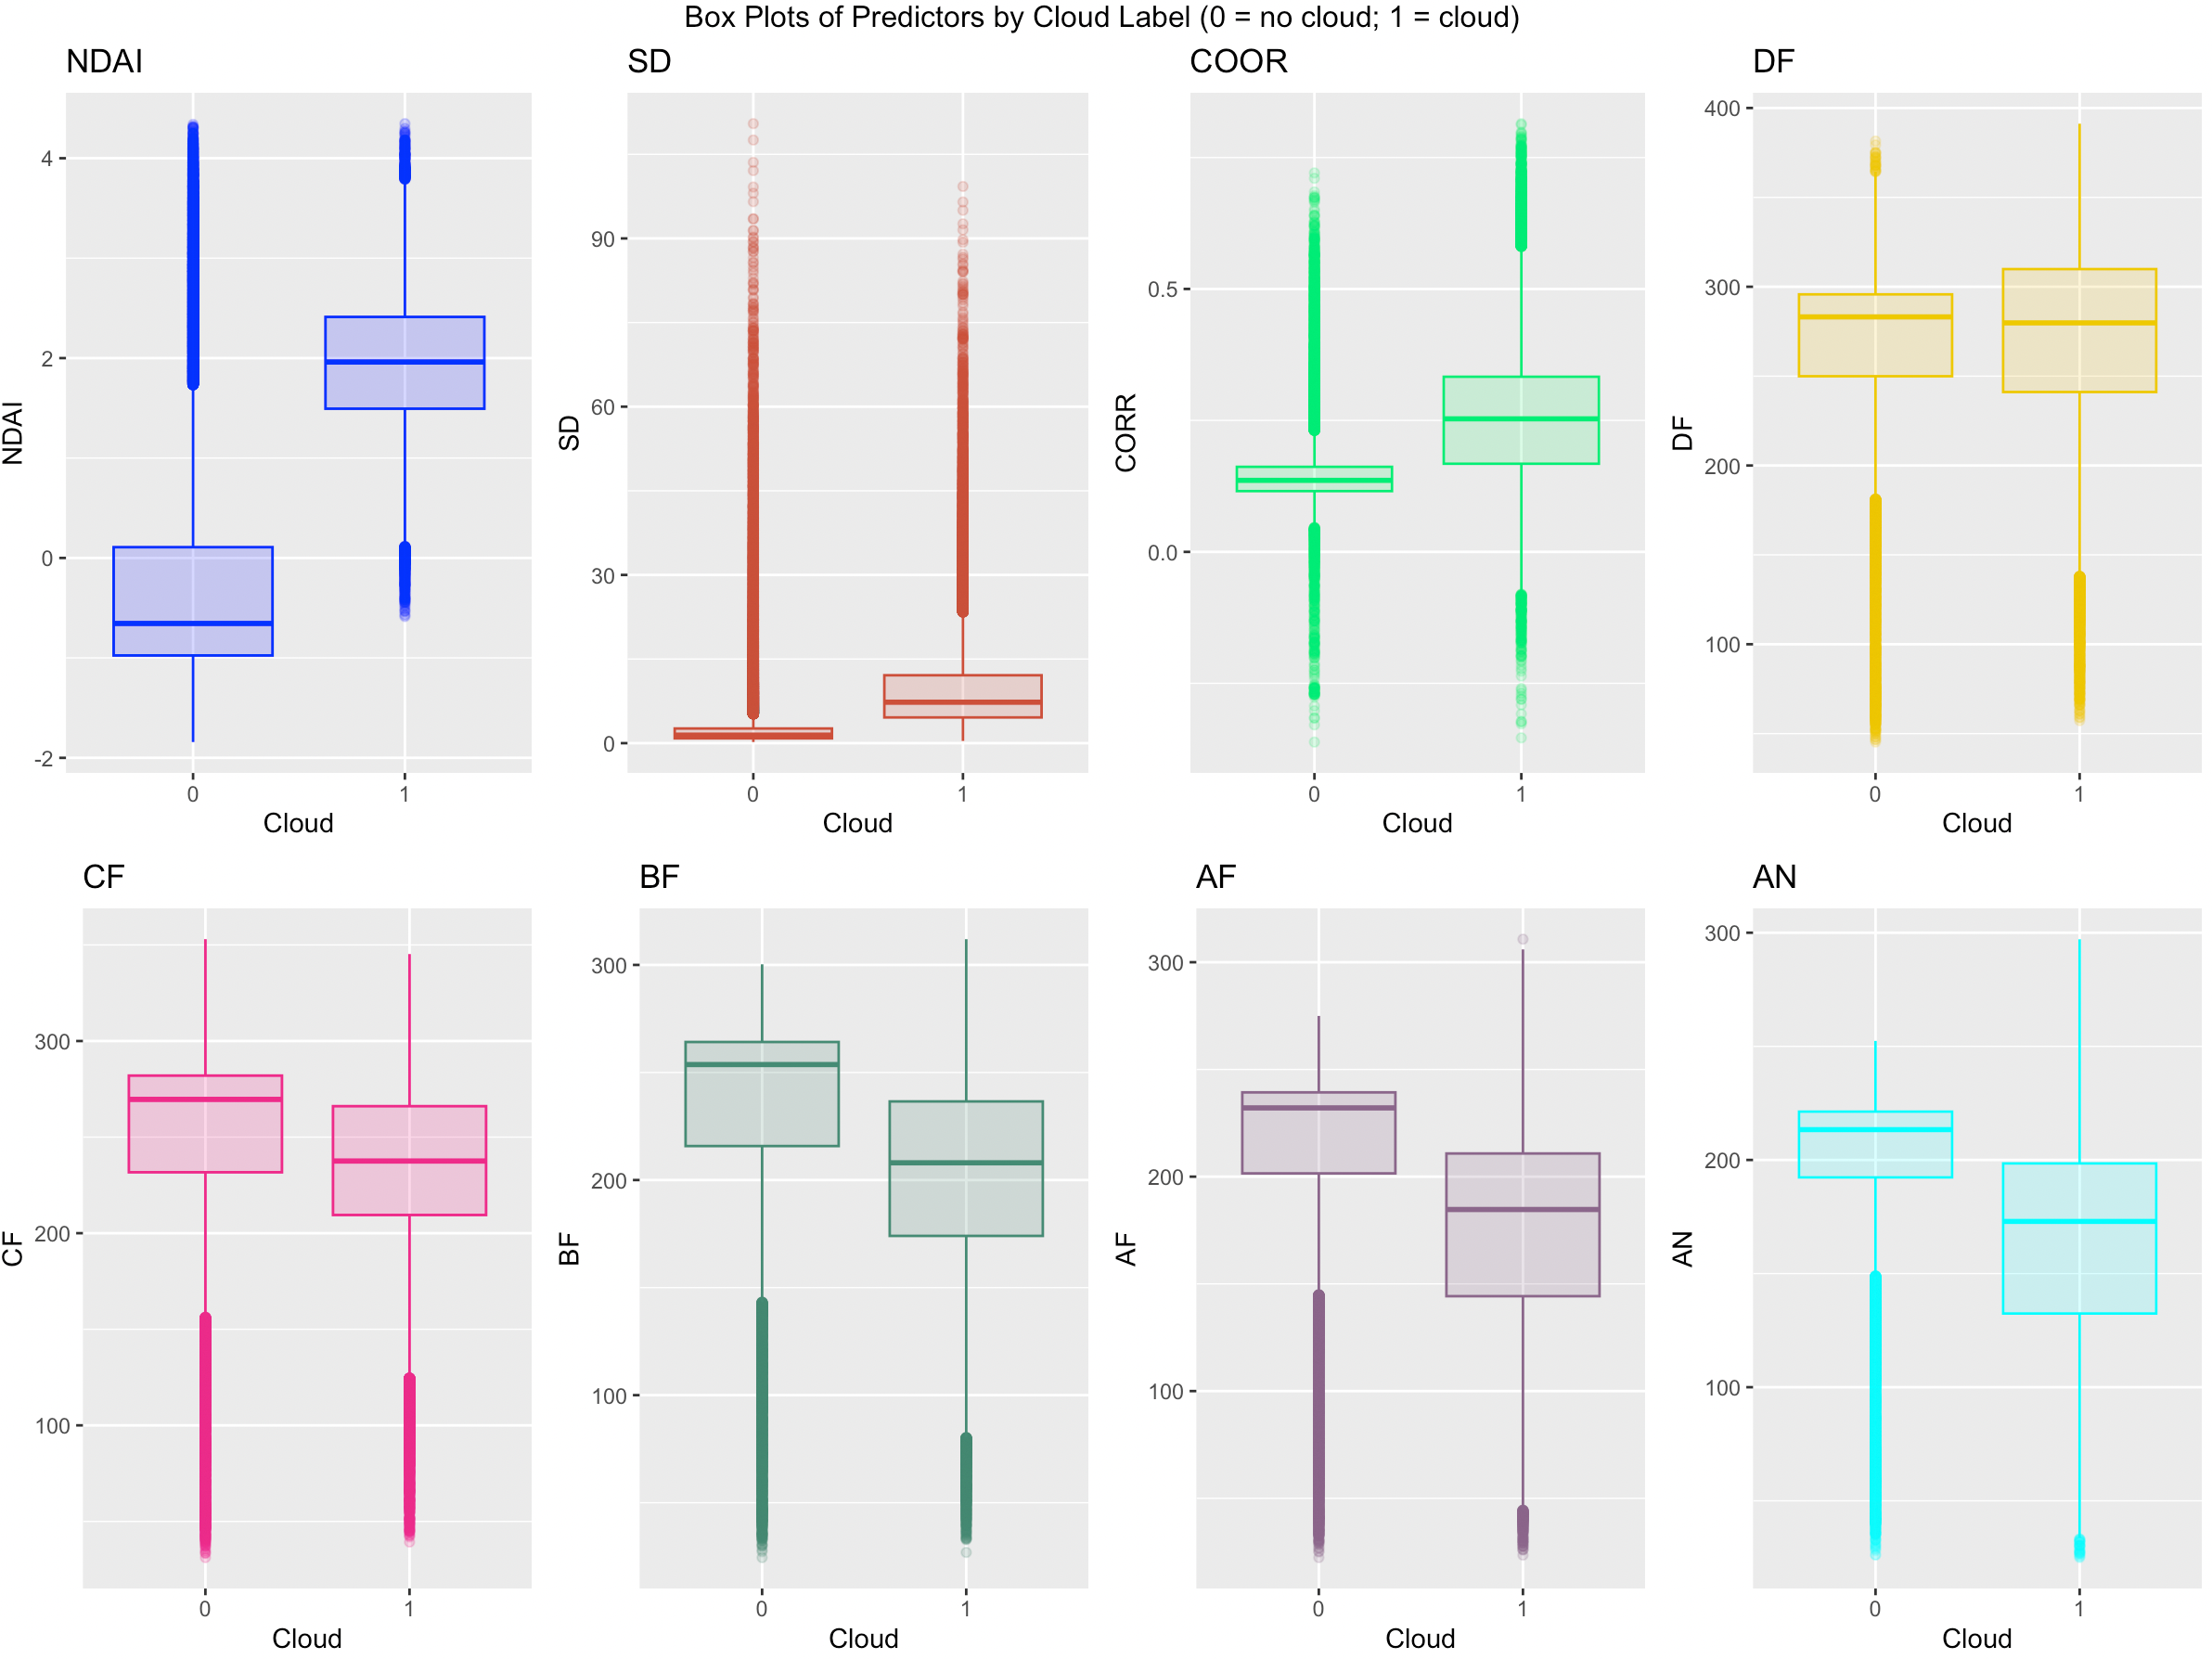
\includegraphics[width=12cm]{Fig3.png}
\centering
\end{figure}
The box plots do appear to be helpful in determining plausibly important predictors of cloud label. Interestingly, NDAI appears to be have visually distinct distributions for non-cloud and could observations. It is clustered around a value of -1 or so when the label is no-cloud; and clustered around 2 when the label is cloud. Substantively, NDAI is a subject-matter expertise variable that captures how a particular surface changes when using various MISR viewing directions of the same surface. NDAI and the cloud label are positively correlated, suggesting that a higher NDAI indicates the presence of a cloud, while lower values indicate no cloud. The distribution of CORR also appears to be different for non-cloud and cloud observations, although less dramatically so. CORR is also a measurement derived from subject matter expertise that shows the correlation between the satellite images of the same scene taken from different angles. This is also positively related to the presence of a cloud: the more correlated the images from different angles are, the more likely it is for an observation to be a cloud. While SD (the third expert-derived measurement) had the substantively largest coefficient in the linear probability model of the remaining predictors, its non-cloud and cloud distributions appear relatively similar, so we do not include it in our model. The various angle variables visually appear to have more distinct distributions---AF and AN both represent good options, as values for non-clouds appear to be concentrated above 200, but more evenly distributed for cloud observations. The Angle AN appears to be the most distinct and is substantively different as it is the only downwards facing camera, so we choose to include this as a third predictor variable in our classifier. With two partition methods, a baseline classification success rate, and three theoretically and empirically justifiable predictor variables in hand, we can now turn to classifier construction, testing, and comparison. 

\section{Modeling}
In order to find the most appropriate classification method to accurately distinguish between cloud and non-cloud data, we try four different classification methods---logistic regression, linear discriminant analysis (LDA), quadratic discriminant analysis (QDA) and decision tree (DT). Using a cross-validation approach, we model the four methods using both of our data partitioning strategies. 

\subsection{Assumptions}
Important assumptions that will impact their accuracy underlie each of these methods. Logistic regression assumes decision boundary to be a hyperplane, which is a very strict assumption clearly not met in this case as the data are obviously not linearly separable. LDA models the data within each class as normal distributed with a common covariance matrix and assumes that the decision boundary is also a hyperplane. Similar to LDA, the QDA classifier results from assuming that observations are drawn from a Gaussian distribution and plug estimates into Bayes' Theorem to preform prediction. Unlike LDA, QDA assumes that each class has its own covariance matrix, allowing a bit more flexibility. LDA tends to be a better bet than QDA if there are relatively few training observations, in contrast QDA is recommended if the training set is large or if the assumption of a common covariance matrix for each of the classes is clearly not possible. In this case, it is reasonable to expect that QDA will produce the best results, followed by LDA and logistic regression. Unlike the previously mentioned methods, there is no probabilstic model that underlies decision trees, and is rather simply a binary split. Therefore, we do not need to rely on strict assumptions for this technique. Given our particular case, the efficacy of this model could go either way---on one hand, it is more flexible not bound by the strict assumptions as the other models, but on the other, decision trees are prone to overfitting to the training data, resulting in low accuracy.   

\subsection{Results}
The accuracy of our classification and partitioning methods varied considerably. The results of the 8 models (4 classification methods for each of the 2 partitioning methods) are recorded in Table 3. First, note that all 8 models significantly outperform the trivial, baseline classifier. Across the board, we see that the horizontal slicing (HS) method performed better than the block partitioning method, usually by several percentage points. This is somewhat intuitive, as we are capturing more spatial variation in slices. For HS methods, test accuracy ranges from 89.9 percent for the logistic regression to 90.9 percent for the decision tree model. LDA and QDA ranked in the middle at 90.8 and 90.3 percent respectively. In contrast, for block partitioning methods, test accuracy ranges from 84 percent for the logistic regression to 87.4 percent for the decision tree. Again, LDA and QDA rank in the middle at 89.8 percent and 89.9 percent respectively. In sum, the horizontal slicing performed better than block partitioning, and decision tree models produced the most accurate test results, followed by LDA, QDA, and logistic regression. The fact that the decision tree model performed the best is rather surprising as trees generally do not have the same level as predictive accuracy as some of the other approaches. Perhaps this is related to the fact we are working with spatial data. However, note that the LDA horizontal slicing model's test error is 90.8 versus the decision tree's 90.9, so the difference is marginal. We will discuss this further in the following section. 
\begin{table}[htp!]
    \centering
    \caption{Model Performance (Accuracy Rate)}
  \footnotesize
\begin{tabular}{@{\extracolsep{5pt}} ccccccccc} 
\\[-1.8ex]\hline 
\hline \\[-1.8ex] 
 & Log HS & Log Block & LDA HS & LDA Block & QDA HS & QDA Block & DT HS & DT Block \\ 
\hline \\[-1.8ex] 
F1 & $0.661$ & $0.913$ & $0.661$ & $0.981$ & $0.670$ & $0.979$ & $0.607$ & $0.847$ \\ 
F2 & $0.919$ & $0.860$ & $0.925$ & $0.864$ & $0.949$ & $0.822$ & $0.938$ & $0.809$ \\ 
F3 & $0.958$ & $0.932$ & $0.960$ & $0.807$ & $0.954$ & $0.877$ & $0.972$ & $0.966$ \\ 
F4 & $0.858$ & $0.955$ & $0.870$ & $0.921$ & $0.859$ & $0.978$ & $0.901$ & $0.962$ \\ 
F5 & $0.917$ & $0.833$ & $0.925$ & $0.918$ & $0.923$ & $0.839$ & $0.943$ & $0.905$ \\
\hline \\[-1.8ex] 
Overall CV & $0.863$ & $0.899$ & $0.868$ & $0.898$ & $0.871$ & $0.899$ & $0.872$ & $0.898$ \\ 
Test & $0.899$ & $0.840$ & $0.908$ & $0.845$ & $0.903$ & $0.848$ & $0.909$ & $0.874$ \\ 
\hline \\[-1.8ex] 
\end{tabular} 
 
\end{table}
\newline
\noindent Figure 4 plots ROC curves for our models with a cut off value at a standard 0.5. A ROC curve compares the performance of classifiers by displaying the trade-off between getting a low false positive rate and a high true positive rate. The overall performance of a classifier is given by the area under the ROC curve (AUC). An ideal ROC curve will hug the top left corner, so the perfect AUC is 1. In our plots, there is a subtle but definite difference between the two plots---the ROC curves of horizontal slicing model hug the upper left corner more tightly, creating more space under the curve compared to the block partitioning models. Within each plot, there is a relatively small difference between classification methods (1-3 percent) between methods, so the lines appear to be stacked. Note that we do not include decision trees in this plot, as decision trees are designed to produce only a class decision (in this case, cloud or no cloud). When a discrete classifier is applied to a test set, it yields a single confusion matrix, which corresponds to a single ROC \textit{point} (Fawcett, 2006, p.863). 
\begin{figure}[htp]
\caption{ROC Curve Plots}
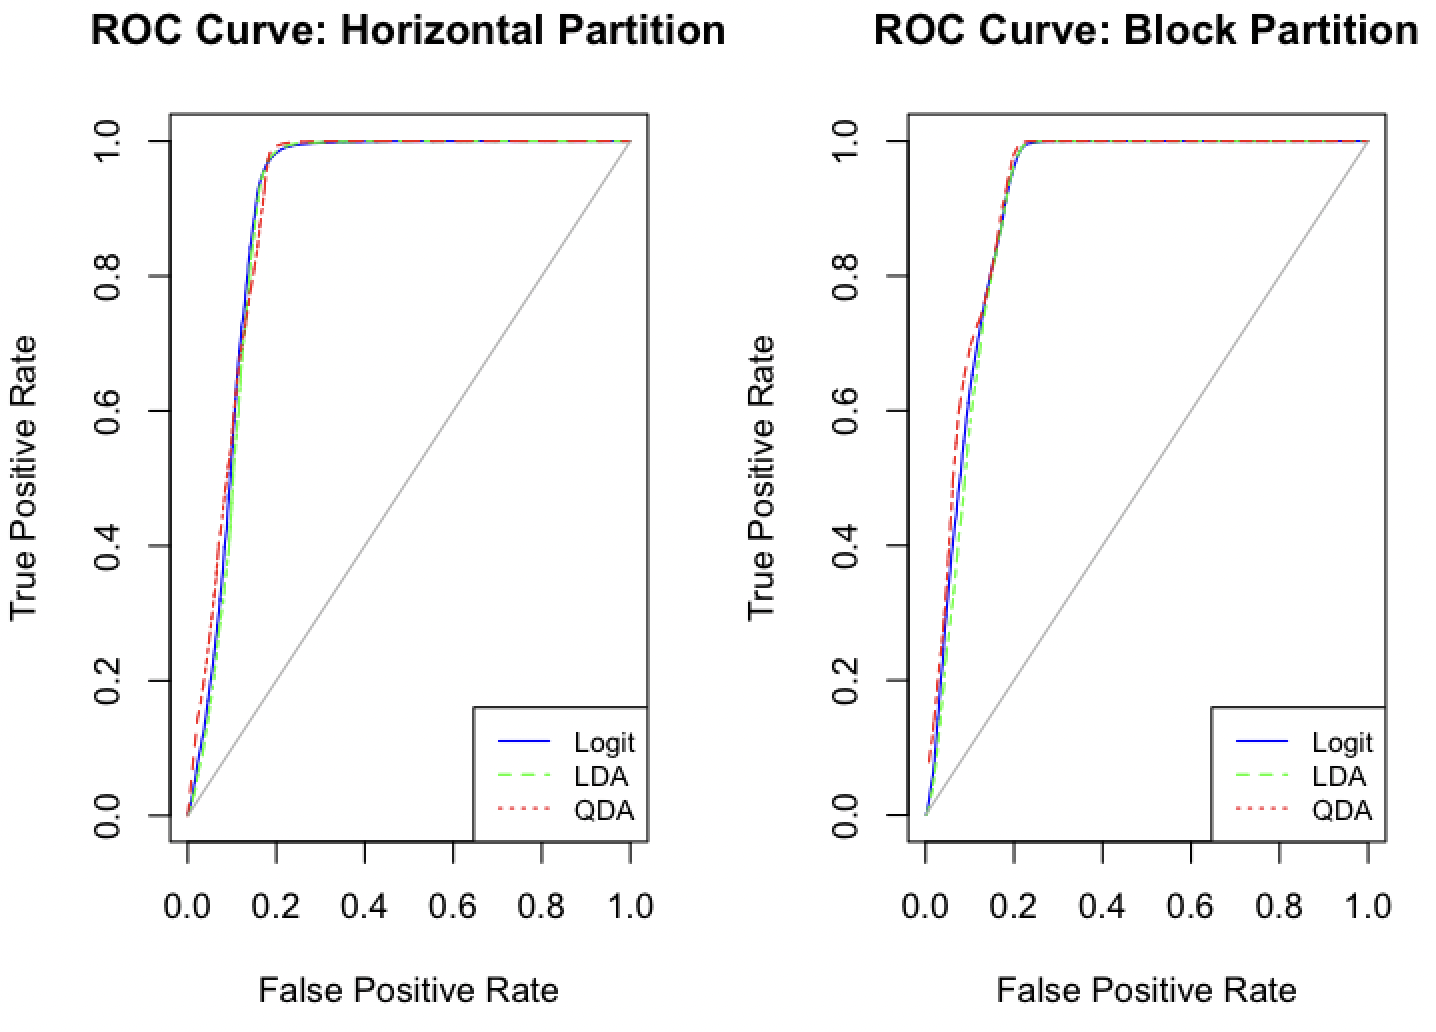
\includegraphics[width=13cm]{Fig4.png}
\centering
\end{figure}
\newline
\newline
\newline
\noindent In addition to ROC curves and the AUC, another metric that would be interesting to examine is the Brier score. A Brier score is a very simple calculation (the mean squared difference between the predicted probability and the actual outcome) that could be especially useful here because it accommodates predictions between 0 and 1. After all, we are constraining three of our classifiers (logit, LDA, and QDA) to providing discrete class predictions (0 or 1), instead of the probabilistic predictions which they can provide. The Brier score punishes overconfidence, so it could allow the more nuanced probabilistic predictions from the logit, LDA, and QDA to outperform the decision tree model by this metric.  Future cloud image analysts might consider calculating and evaluating Brier scores.         

\section{Diagnostics}
\subsection{Confusion Matrices and Performance Metrics}
Now that we have tested all of our models, we will next further evaluate the most promising ones. As we noted, while the horizontal slicing method was clearly more effective than the blocked partition model, there was essentially a tie for most accurate classifier between our decision tree model and our LDA model. We first probe the differences between these two models by creating confusion matrices and examining several standard measures of performance in binary classification problems. In the confusion matrices in Figure 5, we see that the LDA model is slightly better at accurately predicting true negatives, but worse than the decision tree at predicting true positives. The LDA model was better at avoiding false positives, but the biggest discrepancy perhaps stems from the fact that the decision tree model seems to be much better at avoiding false negatives. The LDA model picks up nearly 500 more false positives than the decision tree.  
\newline
\newline
Examining the metrics at the bottom of Figure 5, we also can see that the LDA model is slightly more sensitive, meaning that it is more apt to detecting events in the positive (cloud) class. The decision tree model is more specific, however, indicating that it more exactly detects assignment to the positive class. Finally, we compare kappas, which measure the agreement between the classification and true values. A kappa value of 1 represents perfect agreement. We can see the decision tree's kappa is slightly higher than the LDA model. 
\newline
\newline
Finally, we calculate the F1 scores of the two models. Besides accuracy, the F1 score is another common diagnostic tool that combines precision and recall into one metric by computing the harmonic mean between the two. A model will have a high F1 score if both precision and recall are high. The decision tree model again slightly outperforms the LDA model, with F1 statistics of 0.875 and 0.863 respectively. Taken together, the useful metrics from the confusion matrices show that even though the difference in accuracy between the two models was a mere 0.1, the decision tree model is indeed the better of the two models.  
\begin{figure}[htp!]
\caption{Decision Tree vs. LDA Confusion Matrices}
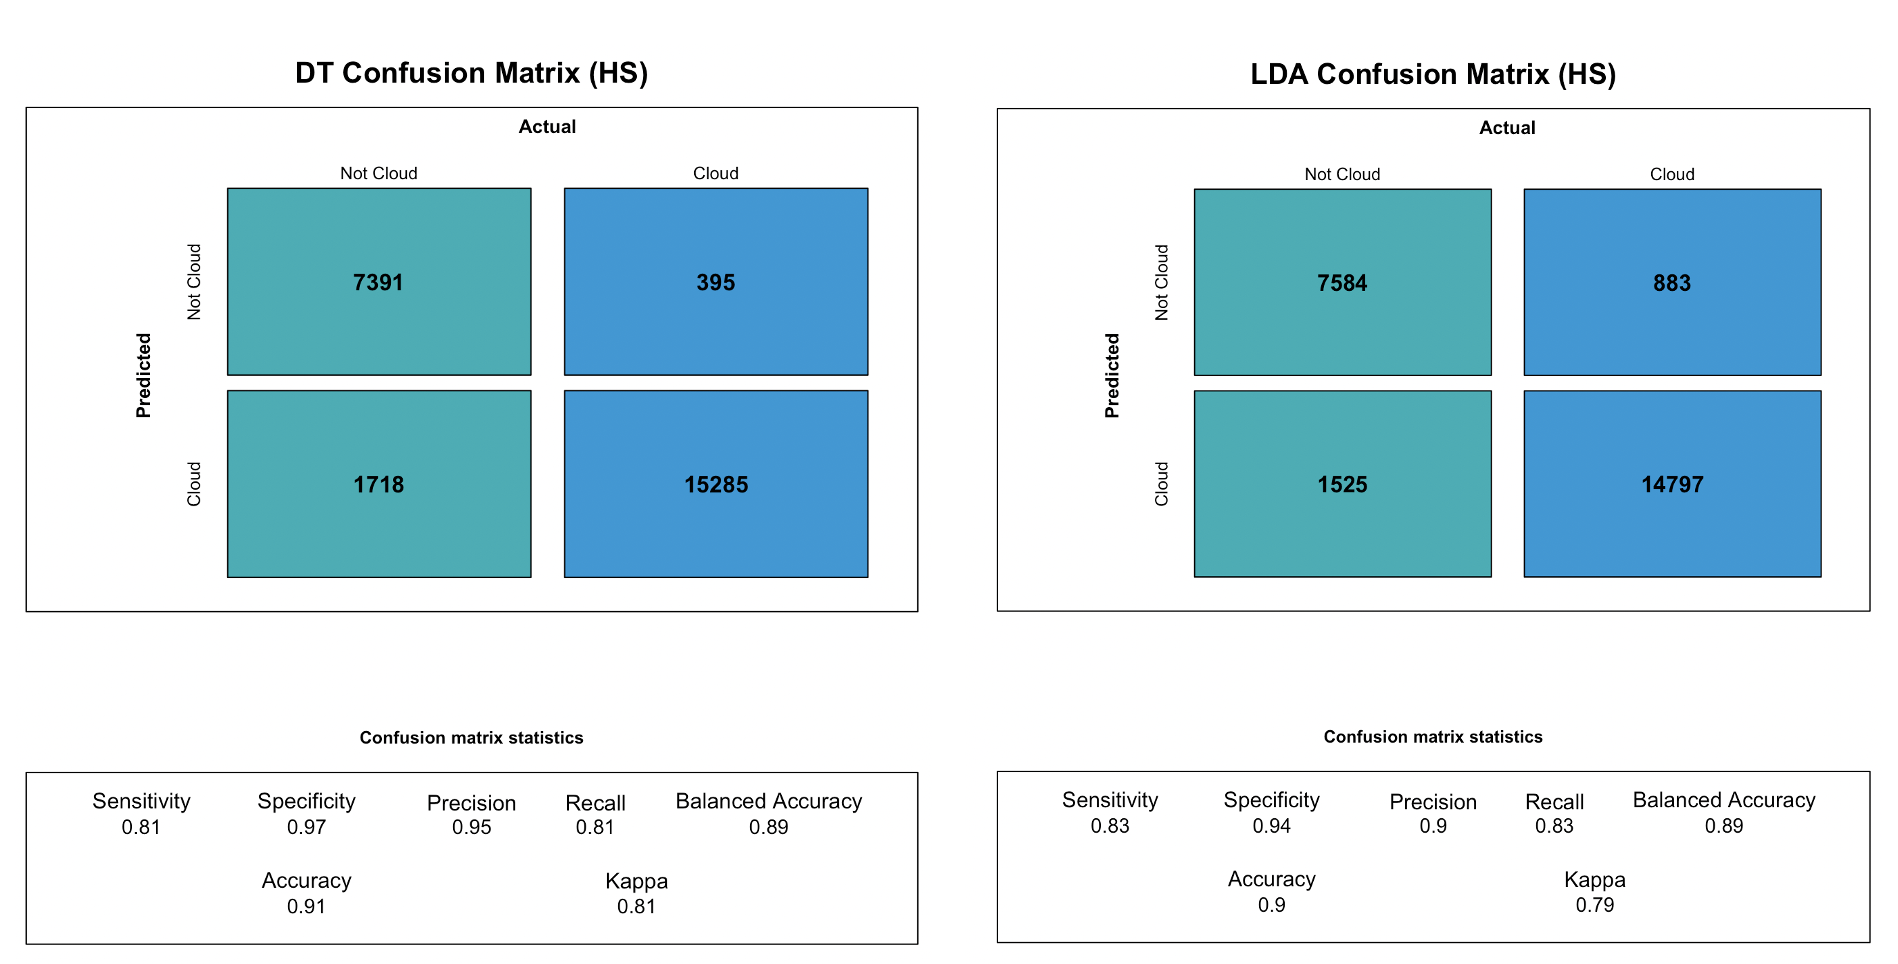
\includegraphics[width=16cm]{Fig5.png}
\centering
\end{figure}
\subsection{Visualizing Decision Tree Predictions}
Now that we have determined that the decision tree model is indeed the most accurate, it is useful to examine patterns in misclassification errors for each of the data partitioning methods. Figure 6 visualizes each of the partitioning methods and plots correct predictions (green), false positives (yellow), and false negatives (red) in one of the three images. In the particular image, we can see that while the horizontal slice method performed very well in some regions, there were others where it did poorly. For example, in the center of the image, the model registered many false positives on a no-cloud segment. With block partitioning, picking up false negatives in the bottom left cloud section of the image seems to be the most significant error. Interestingly, in this particular slice of this particular image, block partitioning appears to perform better than horizontal slicing despite horizontal slicing performing better overall. This illustrates the importance of partitioning method and (re)sampling. 
\begin{figure}[htp!]
\caption{Decision Tree Prediction}
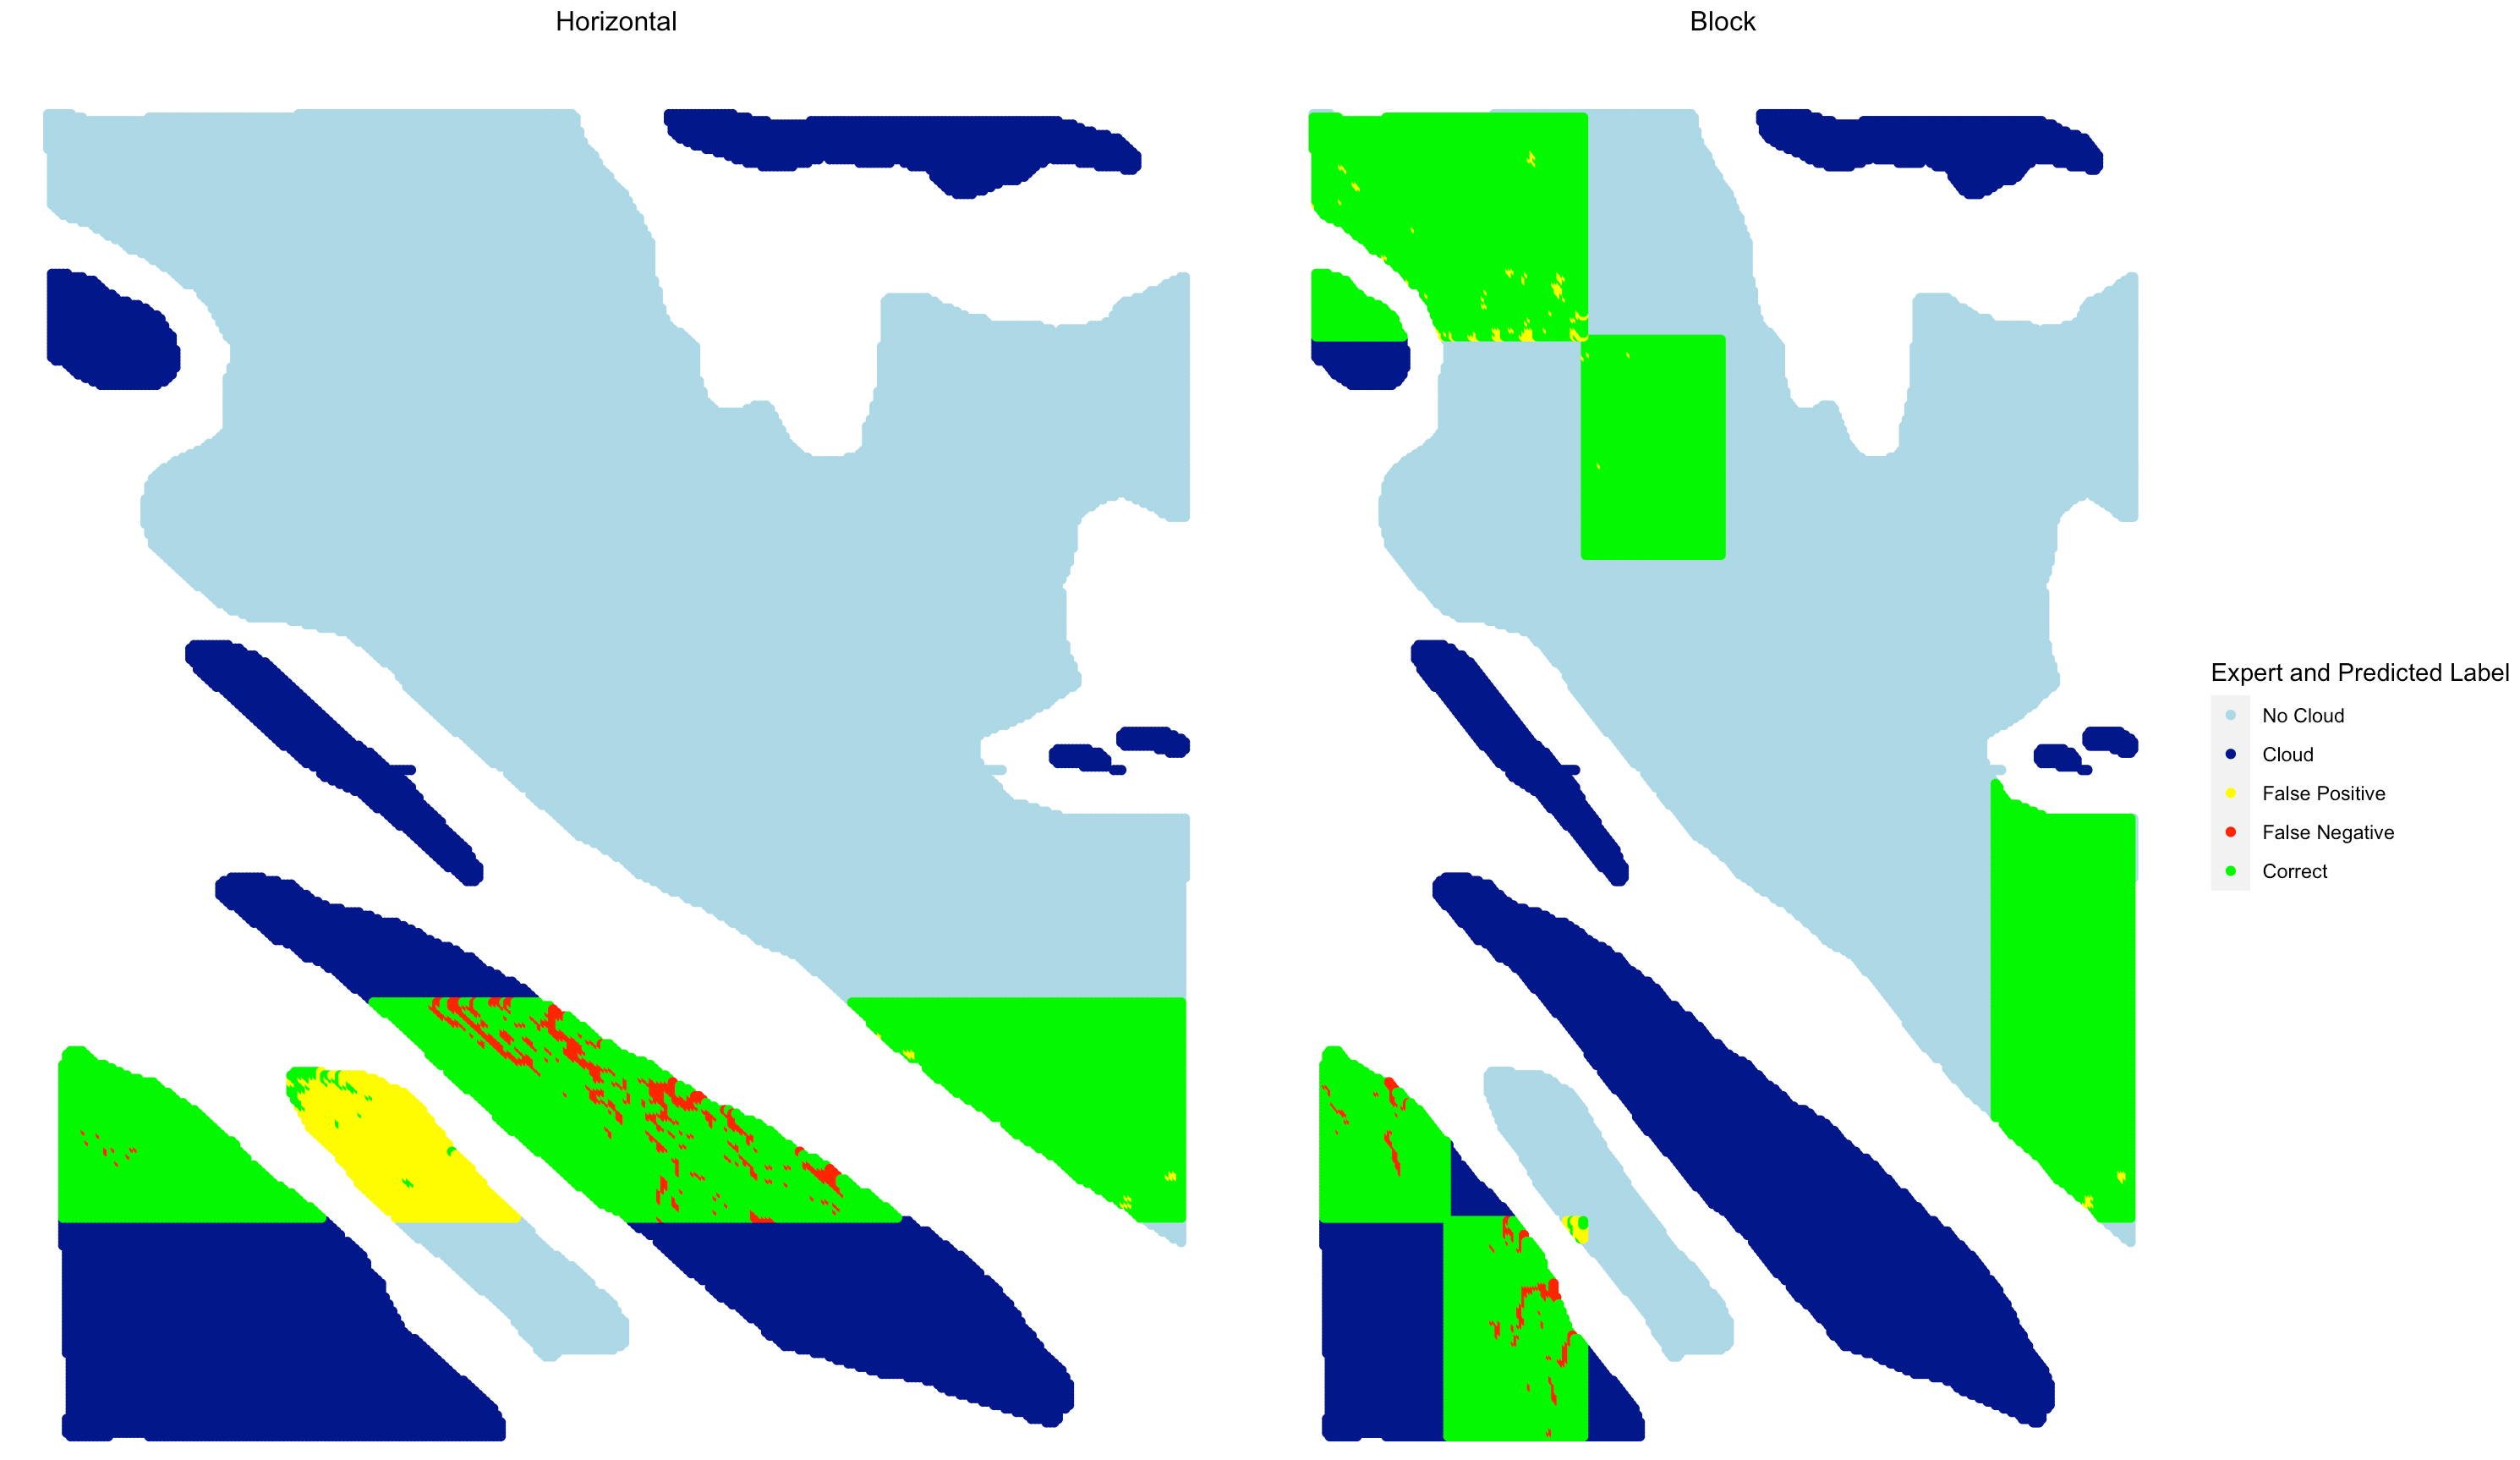
\includegraphics[width=15cm]{Fig6.png}
\centering
\end{figure}
\newline
\newline
Though our decision tree models performed relatively well (91 percent accuracy on test data) with horizontal slice partitioning, there is certainly room for improvement. In this study, we utilize the basic decision tree model, however future researchers may want to apply a more sophisticated tree-based method such as boosting, bagging, or random forest to further improve the performance of the model. Applying bagging or boosting techniques could help decrease the variance of the single-tree estimates by combining several estimates from different models. Ideally, this would result in a model with higher stability. Furthermore, a random forest approach---in which each split on each tree is performed using a random subset of the features, thereby de-correlating the trees, and leading to a potentially more thorough exploration of model space relative to boosting or bagging---also presents an interesting extension for future researchers to explore  (ISL, Ch 8). Notably, these techniques have been applied in similar studies with some success. For example, Avand et al (2020) test tree-based classifcation techniques supplemented by Best First Tree (BFTree), AdaBoost, MultiBoosting, and Bagging to predict the presence of groundwater in the Iranian highlands. In their study---which also uses spatial data to predict the presence of a difficult-to-detect feature---the BFTree-Bagging model had the best performance. Applying these techniques may also help decision tree classifiers perform better in the face of new images without any ground truth.    
\newline
\newline
In conclusion, our analysis shows that while decision tree and LDA methods appear to do relatively well across data partition methods, data visualization of decision tree models show that a more sophisticated tree model could perform even better. Finally, our study illustrates the importance of selecting an appropriate data partitioning method, as there is a large corresponding difference in test accuracy. Most importantly, perhaps, the work by Shi et al (2008) and our subsequent analysis show that rigorous statistical analysis and developing accurate data classification models can contribute to solving some of the most pressing issues facing our planet. 

\section{Replication and Acknowledgements}
The files for reproducing this project can be found in GitHub via our Gradescope submission. We make the following files available: our raw Latex code for reproducing the report including tables and figures; two .R files (one with the general code and one with the CVmaster function), and a README file describing how to reproduce the paper. 
\newline
\newline 
Both authors contributed equally to this project. Viola wrote up most of the analysis, conducted the exploratory data analysis, made most of the visualizations, and compiled the project in Overleaf. Andrew wrote most of the data partitioning functions and CVmaster and worked primarily on the modelling and diagnostic sections, however both authors contributed to all parts. In addition to using class notes, lecture slides, and the ISL textbook, we consulted with several classmates for assistance with various parts of the assignment. In particular, Eli Gnesin, Will Tirone, and Ying Chi helped us conceptualize data partitioning. We also consulted with several of our classmates in the PhD political science program for help with components of functions and de-bugging specific sections of our code. Over the course of working on the project, we referenced many StackExchange threads and other statistics blogs to troubleshoot our code. We also cite the following academic works: 
\newline
\newline
Avand, M., Janizadeh, S., Bui, D., Pham, V., Ngo, P., and Nhu, V., 2020. A tree-based intelligence ensemble approach for spatial prediction of potential groundwater, \textit{International Journal of Digital Earth}, 13(12), 1408--1429.
\newline
\newline
Fawcett, T. 2006. An Introduction to ROC Analysis, \textit{Pattern Recognition Letters}, (27), 861--874. 
\end{document}

